\iffalse
\documentclass[
  bibliography=totoc,     % Literatur im Inhaltsverzeichnis
  captions=tableheading,  % Tabellenüberschriften
  titlepage=firstiscover, % Titelseite ist Deckblatt
]{scrartcl}
\fi





\documentclass{beamer}
\usetheme{Boadilla}


% Paket float verbessern
\usepackage{scrhack}

% Warnung, falls nochmal kompiliert werden muss
%\usepackage[aux]{rerunfilecheck}                       HAB ICH WEG GEMACHT

% unverzichtbare Mathe-Befehle
\usepackage{amsmath}
% viele Mathe-Symbole
\usepackage{amssymb}
% Erweiterungen für amsmath
\usepackage{mathtools}

\usepackage{braket}
\usepackage{nicefrac}

% Fonteinstellungen
\usepackage{fontspec}
% Latin Modern Fonts werden automatisch geladen
% Alternativ:
%\setromanfont{Libertinus Serif}
%\setsansfont{Libertinus Sans}
%\setmonofont{Libertinus Mono}
%\recalctypearea % Wenn man andere Schriftarten gesetzt hat,    HAB ICH WEGGEMACHT
% sollte man das Seiten-Layout neu berechnen lassen

% deutsche Spracheinstellungen
\usepackage{polyglossia}
\setmainlanguage{german}
%\usepackage{ngerman}%ae usw

\usepackage[
  math-style=ISO,    % ┐
  bold-style=ISO,    % │
  sans-style=italic, % │ ISO-Standard folgen
  nabla=upright,     % │
  partial=upright,   % ┘
  warnings-off={           % ┐
    mathtools-colon,       % │ unnötige Warnungen ausschalten
    mathtools-overbracket, % │
  },                       % ┘
]{unicode-math}

% traditionelle Fonts für Mathematik
\setmathfont{Latin Modern Math}
% Alternativ:
%\setmathfont{Libertinus Math}

\setmathfont{XITS Math}[range={scr, bfscr}]
\setmathfont{XITS Math}[range={cal, bfcal}, StylisticSet=1]

% Zahlen und Einheiten
\usepackage[
  locale=DE,                   % deutsche Einstellungen
  separate-uncertainty=true,   % immer Fehler mit \pm
  per-mode=symbol-or-fraction, % / in inline math, fraction in display math
]{siunitx}
\sisetup{mode=text,range-phrase = {\text{~und~}}}

% chemische Formeln
\usepackage[
  version=4,
  math-greek=default, % ┐ mit unicode-math zusammenarbeiten
  text-greek=default, % ┘
]{mhchem}

% richtige Anführungszeichen
\usepackage[autostyle]{csquotes}

% schöne Brüche im Text
\usepackage{xfrac}

% Standardplatzierung für Floats einstellen
\usepackage{float}
\floatplacement{figure}{htbp}
\floatplacement{table}{htbp}

% Floats innerhalb einer Section halten
\usepackage[
  section, % Floats innerhalb der Section halten
  below,   % unterhalb der Section aber auf der selben Seite ist ok
]{placeins}

% Seite drehen für breite Tabellen: landscape Umgebung
\usepackage{pdflscape}

% Captions schöner machen.
\usepackage[
  labelfont=bf,        % Tabelle x: Abbildung y: ist jetzt fett
  font=small,          % Schrift etwas kleiner als Dokument
  width=0.9\textwidth, % maximale Breite einer Caption schmaler
]{caption}
% subfigure, subtable, subref
\usepackage{subcaption}

% Grafiken können eingebunden werden
\usepackage{graphicx}
% größere Variation von Dateinamen möglich
\usepackage{grffile}

% schöne Tabellen
\usepackage{booktabs}

% Verbesserungen am Schriftbild
\usepackage{microtype}

% Literaturverzeichnis
\usepackage[
  backend=biber,
]{biblatex}
% Quellendatenbank
\addbibresource{lit.bib}
\addbibresource{programme.bib}

\iffalse
% Hyperlinks im Dokument
\usepackage[
  unicode,        % Unicode in PDF-Attributen erlauben
  pdfusetitle,    % Titel, Autoren und Datum als PDF-Attribute
  pdfcreator={},  % ┐ PDF-Attribute säubern
  pdfproducer={}, % ┘
]{hyperref}
\fi                                            %HYPERREF HAB ICH WEGGEMACHT
% erweiterte Bookmarks im PDF
%\usepackage{bookmark}                            HAB ICH WEGGEMACHT



% Trennung von Wörtern mit Strichen
\usepackage[shortcuts]{extdash}




\title{My Presentation}
\subtitle{Using Beamer}
\author{Ismael Abu Dabi}
\institute{Technische Universit"at Dortmund}
\date{\today}



\iffalse
\subject{V27}
\title{Zeeman Effekt}
\date{
  Durchführung: 09. Juli 2018
  \hspace{3em}
  Abgabe: 08.08.2018
}

\begin{document}

\maketitle
%\thispagestyle{empty}
\tableofcontents
\newpage

\section{Zielsetzung}
  Im Versuch wird die, durch den (an)normalen Zeeman-Effekt versuchsachte, Aufspaltung der Energieniveaus von Cadmium (Cd) mit einem geeigneten Versuchsaufbau visualisiert und die experimentel ermittelten Energiedifferenzen mit den theoretisch berechneten verglichen.


\section{Theorie}
\label{sec:Theorie}
  Als Zeeman-Effekt wird das Phenomen bezeichnet, dass sich die diskreten Energieniveaus der Elektronen in Atomen unter Einfluss eines "au"seren Magnetfeldes $\vec{B}$ aufspalten.
  Es wird zwischen normalem und annormalem Zeeman-Effekt unterschieden.


  \subsection{Magnetisches Moment von Atomen}
    Wegen der Ladung des Elektrons entstehen druch dessen Drehimpuls $\vec{l}$ bzw. Spin $\vec{s}$ magnetische Momente $\vec{\mu_l}$ und $\vec{\mu_s}$.
    Mit den quantenmechanischen Erwartungswerten f"ur $l^2$ und $s^2$ folgen f"ur die Betr"age der mafgnetischen Momente:
    \begin{align}
      \begin{split}
        |\vec{\mu_l}| &= \mu_l = -\mu_B\sqrt{l(l+1)} \\
        |\vec{\mu_s}| &= \mu_s = -g_s\mu_B\sqrt{s(s+1)}
      \end{split}
    \end{align}
    Dabei ist
    \begin{equation}
      \mu_B = -\frac{1}{2}e\frac{\hbar}{m_e}
    \end{equation}
    das sogenannte Bohr'sche Magneton und $g_s \approx 2$ ist der Lande-Faktor des Elektrons.
    $l = 0,1,2,...,n-1$ (mit der Hauptquantenzahl $n$) und $s=\frac{1}{2}$ sind die Drehimpuls- und Spin Quantenzahl des Elektrons.

    Um das magnetische Moment eines Atoms zu bestimmen, muss man nur die magnetischen Momente (druch Drehimpuls und Spin) der Elektronen der "au"seren Schale/Energieniveau ber"ucksichtigen, da sich der Gesamtspin und -drehimpuls von abgeschlossenen Schaalen nach den Hund'schen-Regeln zu 0 addieren.

    F"ur die vorliegende Situation, dass die Ordungszahl des Atoms und angelegte "au"sere Magnetfelder nicht zu gro"s sind, kann angenommen werden, dass sich die Spins und Bahndrehimpulse aller beteiligten Elektronen vektoriell zum Gesamtdrehimpuls und Gesamtspin addieren
    \begin{align}
      \begin{split}
        S &= \sum s_i\\
        L &= \sum l_i \; ,
      \end{split}
    \end{align}
    womit f"ur die magnetischen Momente gilt
    \begin{align}
      \begin{split}
        |\vec{\mu_L}| &= \mu_L = -\mu_B\sqrt{L(L+1)} \\
        |\vec{\mu_S}| &= \mu_S = -g_S\mu_B\sqrt{S(S+1)} \; .
      \end{split}
    \end{align}
    $S$ und $L$ sind nun die Quantenzahlen des Atoms.

    Da sich der Gesamtdrehimpuls $J$ durch $J=L+S$ ergibt, folgt f"ur das gesamte magnetische Moment des Atoms
    \begin{align}
      \begin{split}
        \mu_J = \mu_L + \mu_S = g_J \mu_B \sqrt{J(J+1)}
      \end{split}
    \end{align}
    mit dem Lande-Faktor $g_J$ des betreffenden Atoms:
    \begin{equation}
      g_J = \frac{3J(J+1) + S(S+1) - L(L+1)}{2J(J+1)} = 1 \; \text{f"ur S=0}
      \label{g_J}
    \end{equation}


  \subsection{Zeeman-Effekt}
    Hat ein Atom das magnetische Moment $\mu_J$, erh"ahlt dieses die zus"atzliche Energie
    \begin{equation}
      E_{mag} = -\vec{\mu_J} \cdot \vec{B}
    \end{equation}
    im Magnetfeld $\vec{B}$.

    Es k"onnen nur Winkel zwischen $\vec{\mu_J}$ und $\vec{B}$ auftreten (Richtungsquantelung) bei denen f"ur die Komponente $\mu_{{J_z}||}$ parallel zur Feldrichtung gilt:
    \begin{equation}
      \mu_{{J_z}||} = -mg_J\mu_B\;,\;, -J \leq m \leq J
    \end{equation}
    Daraus folgt
    \begin{equation}
      E_{mag} = mg_J\mu_BB \; .
    \end{equation}
    Die Energiedifferenz zweier durch den Zeeman-Effekt aufgespaltenen Energieniveaus/Zust"ande ist daher
    \begin{equation}
    \delta E = (m_ig_{J,i}-m_jg_{J_j})\mu_BB = g_{ij} \mu_BB \; .
    \label{g_ij} 
    \end{equation}
    %mit der Energiedifferenz ohne B-Feld $\delta E_0$.
    $g_{ij}$ ist folglich der Lande-Faktor des "Ubergangs $i \leftrightarrow j$.
    %$\delta E$ ist genau die Energie des Photons, das beim "Ubergang zwischen dem Zustand/der Wellenfunktion $\Psi_i$ und $\Psi_j$ ausgestrahlt wird.

  %  F"ur $S =0$ (normaler Zeeman-Effekt) ist $g_J=1$ und
  %  \begin{equation}
  %    E_{mag} =  m\mu_BB .
  %  \end{equation}
  %  F"ur $S \neq 0$ (annormaler Zeeman-Effekt) gilt

\iffalse
  \subsection{Der Zeeman-Effekt}
    Hat ein Atom ein magnetisches momen mue, wird erhaelt dieses zus"atzliche energie Emag=-mujB im aeusseren magnetfeld.
    res koennen nur winkel zwischen mue und b auftreten koennen. bei denen mujz =  ist (Richtungsquantelung), m ist debei element -j bis j.
    Damit wird e mag zu :

    F"ur S=0 ist gj immer 1 (normaler zeeman effekt), fuer s =/= ist gj = ... - gji (annormaler zeeman effekt)
\fi



  \subsection{Auswahlregeln f"ur die Quantenzahl $m$ bei den "Uberg"angen mit Zeeman-Effekt}
    Durch Betrachtung der "Ubergangswahrscheinlichkeit zwischen dem Zustand $\Psi_1$ und $\Psi_2$ zeigt sich, dass nur "Uberg"ange mit
    \begin{equation}
      \Delta m = m_1 - m_2= \pm1,0
    \end{equation}
     m"oglich sind.
    "Uberg"ange mit $\Delta m = 0$ ($\pi$-"Uberg"ange) emittieren lineares, parallel zu $\vec{B}$ polarisiertes Licht.
    Bei "Uberg"angen mit $\Delta m = \pm 1$ ($\sigma$-"Uberg"ange) wird zirkular um die B-Feld-Achse polarisiertes Licht erzeugt.

  \subsection{"Uberg"ange der Cadmium Lampe}
    Im Experiment werdem der normale und annormale Zeeman-Effekt verifiziert, indem die Spektraliniern Aufspaltung einer Cadmium-Lampe im Magnetfeld visualisiert wird.
    Es werden die zwei "Uberg"ange $^1P_1 \leftrightarrow ^1D_2$ (rotes Licht mit $\lambda = \SI{643,8}{\nano \meter}$, normaler Zeeman-Effekt) und $^1S_1 \leftrightarrow ^3P_1$ (blaues Licht mit $\lambda = \SI{480,0}{\nano \meter}$, annormaler Zeeman-Effekt) untersucht, welche sich nach dem Anglegen des Magnetfeldes nach dem Zeeman-Effekt aufspalten.

    Die theoretischen Lande-Faktoren der einzelnen Energie-Niveaus $g_1$ und $g_2$ sowie die Lande-Faktoren $g_{ij}$ der $\pi$- und $\sigma$-"Uberg"ange sind f"ur den urspr"unglichen $^1P_1 \leftrightarrow ^1D_2$ "Ubergang sind in Tabelle (\ref{rot}) und f"ur den urspr"unglichen $^1S_1 \leftrightarrow ^3P_1$ "Ubergang  in Tabelle (\ref{blau}) dargestellt.
    Die $g_{1,2}$ werden nach Formel (\ref{g_J}) berechnet.

    \begin{table}
    	\centering
    	\begin{tabular}{c|cc|cc|c}
    		%\toprule
    		Übergang & $m_1$  & $g_{1}$ & $m_2$ & $ g_2$ & $g_{12}$\\
    		\midrule
    		& \multicolumn{2}{c}{${}^1P_1$}  & \multicolumn{2}{c}{${}^1D_2$} \\
    		\midrule
    		& 2 & 1 & 1 & 1 & 1\\
    		$\sigma$& 1 & 1 & 0 & 1 & 1\\
    		& 0 & 1 & -1 & 1 & 1\\
    		\midrule
    		& 1 & 1 & 1 & 1 & 0\\
    		$\pi$ & 0 & 1 & 0 & 1 & 0\\
    		& -1 & 1 & -1 & 1 & 0\\
    		\midrule
    		& 0 & 1 & 1 & 1 & -1\\
    		$\sigma$ & -1 & 1 & 0 & 1 & -1\\
    		& -2 & 1 & -1 & 1 & -1\\\bottomrule
    	\end{tabular}
    	\caption{Lande-Faktoren f"ur den roten "Ubergang.}
    	\label{rot}
    \end{table}
    \begin{table}
    	\centering
    	\begin{tabular}{c|cc|cc|c}
    		%\toprule
    		Übergang & $m_1$  & $g_{1}$ & $m_2$ & $ g_2$ & $g_{12}$\\
    		\midrule
    		& \multicolumn{2}{c}{${}^3S_1$}  & \multicolumn{2}{c}{${}^3P_2$} \\
    		\midrule
    		$\sigma$ & +1 & 2 & 0 & $\frac{3}{2}$& 2\\
    		& 0 & 2 & -1 & $\frac{3}{2}$ & $\frac{3}{2}$\\
    		\midrule
    		& +1 & 2 & +1 & $\frac{3}{2}$ & $\frac{1}{2}$\\
    		$\pi$ & 2 & 2 & 0 & $\frac{3}{2}$ & 0 \\
    		& -1 & 2 & -1 & $\frac{3}{2}$ & -$\frac{1}{2}$\\
    		\midrule
    		& 0 & 2 & 1 & $\frac{3}{2}$ & -$\frac{3}{2}$\\
    		$\sigma$ & -1 & 2 & 0 & $\frac{3}{2}$& -2\\
    		\bottomrule
    	\end{tabular}
    	\caption{Lande-Faktoren f"ur den blauen "Ubergang.}
    	\label{blau}
    \end{table}



    .

\section{Durchführung}
\label{sec:Durchführung}
\begin{figure}[h]
	\centering
	\includegraphics[width=14cm,height=11cm]{fotos/Bilddurchfuhrung1.pdf}
	\caption{Schematischer Aufbau der Messapparatur}
	\label{durch:1}
\end{figure}
Zuerst soll eine Vorbereitungsaufgabe gelöst werden, um mit der Durchführung beginnen zu können.
Als erstes wird die Cd-Lampe mit einem Objektiv und einer Linse $L1$ so eingestellt, dass sie scharf auf den Spalt $S1$ abbildet. Im nächsten Schritt wird die Linse $L2$ justiert, sodass ein paralleles Lichtbündel auf das Glasprisma fällt. Um Strahlungsverluste zu vermeiden, wird der Durchmesser des Lichtbündels möglichst klein gehalten. Desweiteren soll der erste Schritt aus der Durchführung für die Linse $L3$ und den Spalt $S2$ wiederholt werden. Es soll nun möglich sein mit diesem Bild eine Wellenlänge auszuwählen. Nun soll mittels der Linse $L4$ ein scharfes Bild auf die Lummer-Gehrcke-Platte abgebildet werden. Beim nächsten Schritt wird die Polarisation je nach Versuchsteil auf $0^{\circ}$ bzw. $90^{\circ}$ eingestellt. Zuletzt wird das Magnet eingeschaltet um die Zeeman-Linien zu beobachten. Als letztes wird das Bild mit einer Digitalkamera aufgenommen und gespeichert.



\section{Auswertung}
\label{sec:Auswertung}




  \subsection{Eichung des Elektromagneten}
  In Tabelle \ref{tab:mit} sind die eingestellten Stromstärken $I$ und die mit einer Hallsonde gemessenen zugehörigen Magnetfeldstärken $B$ aufgelistet.
  
  \begin{table}[H] 
	\centering
	\caption{Für die Eichung des Magneten aufgenommene Messwerte des Magnetfeldes neben der zugehörigen Stromstärke} 
	\begin{tabular}{c|c}

Strom I / A & Magnetische Flussdichte B \\ 
\hline 
1	& 60 \\
2	& 123 \\
4	& 236\\
6	& 330\\
8	& 460\\
10	& 580\\
12	& 700\\
14	& 800\\
16	& 890\\
18	& 960\\
20	& 1020\\	
		
	\end{tabular} 
	  \label{tab:mit}
\end{table} 

\begin{figure}[h]
	\centering
	\includegraphics[width=12cm,height=8cm]{plot/V27_plot_1.pdf}
	\caption{Magnetischer Flussdichte gegen Stromstärke aufgetragen}
	\label{plot:1}
\end{figure}

Mit den Messwerten aus Tabelle \ref{tab:mit} wird eine Ausgleichsrechnung mittels der Funktion 
\begin{align}
f(x)= ax+b
\end{align}

durchgeführt. Für die Parameter erhält man durch den Fit:

\begin{center}
a = 52,4581 \pm 1,512 $\frac{mT}{A}$
\\
b = 30,5592 \pm 17,9 $mT$

\end{center}    



  \subsection{\texorpdfstring{Aufl"oseverm"ogen $A$ und Dispersionsgebiet $\Delta \lambda$ der verwendeten Lummer-Gehrcke-Platte f"ur die Wellenl"angen des roten und blauen "Ubergangs}{Aufl"oseverm"ogen A und Dispersionsgebiet Delta lambda der verwendeten Lummer-Gehrcke-Platte f"ur die Wellenl"angen des roten und blauen "Ubergangs}}
  
  Die zur Berechnung notwendigen Größen sind in der Versuchsanleitung gegeben
  
  \begin{center}
  L = 120 mm \\
  d = 4 m \\
  n(644nm) = 1,4567 \\
  n(480nm) = 1,4635. \\
  \end{center}
Das Dispersionsgebiet $\Delta \lambda$ und das Auflösevermögen $A$ wurden mit den folgenden Formeln berechnet und in der Tabelle aufgeführt.
  \begin{equation}
\Delta \lambda_D=\frac{\lambda^2}{2d}\cdot \sqrt{\frac{1}{n^2-1}}
\end{equation}

\begin{equation}
A=\frac{\lambda}{\Delta = \lambda}\frac{L}{\lambda}\Bigl(n^2-1\Bigr)
\end{equation}

  
    \begin{table}[H] 
	\centering
	\caption{Dispersionsgebiet $\Delta \lambda$ und das Auflösevermögen $A$} 
	\begin{tabular}{c|c|c}

  & rot & blau\\ 
\hline 
$\lambda$	 		& 643,8 nm & 480 nm \\
$\Delta \lambda $	& 48,91 pm & 26,95 pm \\
A				& 209129 & 285458 \\

		
	\end{tabular} 
	  \label{tab:mit2}
\end{table} 
  \newpage
    \subsection{\texorpdfstring{Bestimmung des Lande-Faktors $g_{12}$ der $\sigma$-"Uberg"ange f"ur die rote Linie}{Bestimmung des Lande-Faktors g_{12} der sigma-"Uberg"ange f"ur die rote Linie}}
    
    Für die rote Spektrallinie der Wellenlänge $\lambda = 643.8 nm$ wurden folgende Bilder aufgenommen werden
    
    \begin{figure}[h]
	\centering
	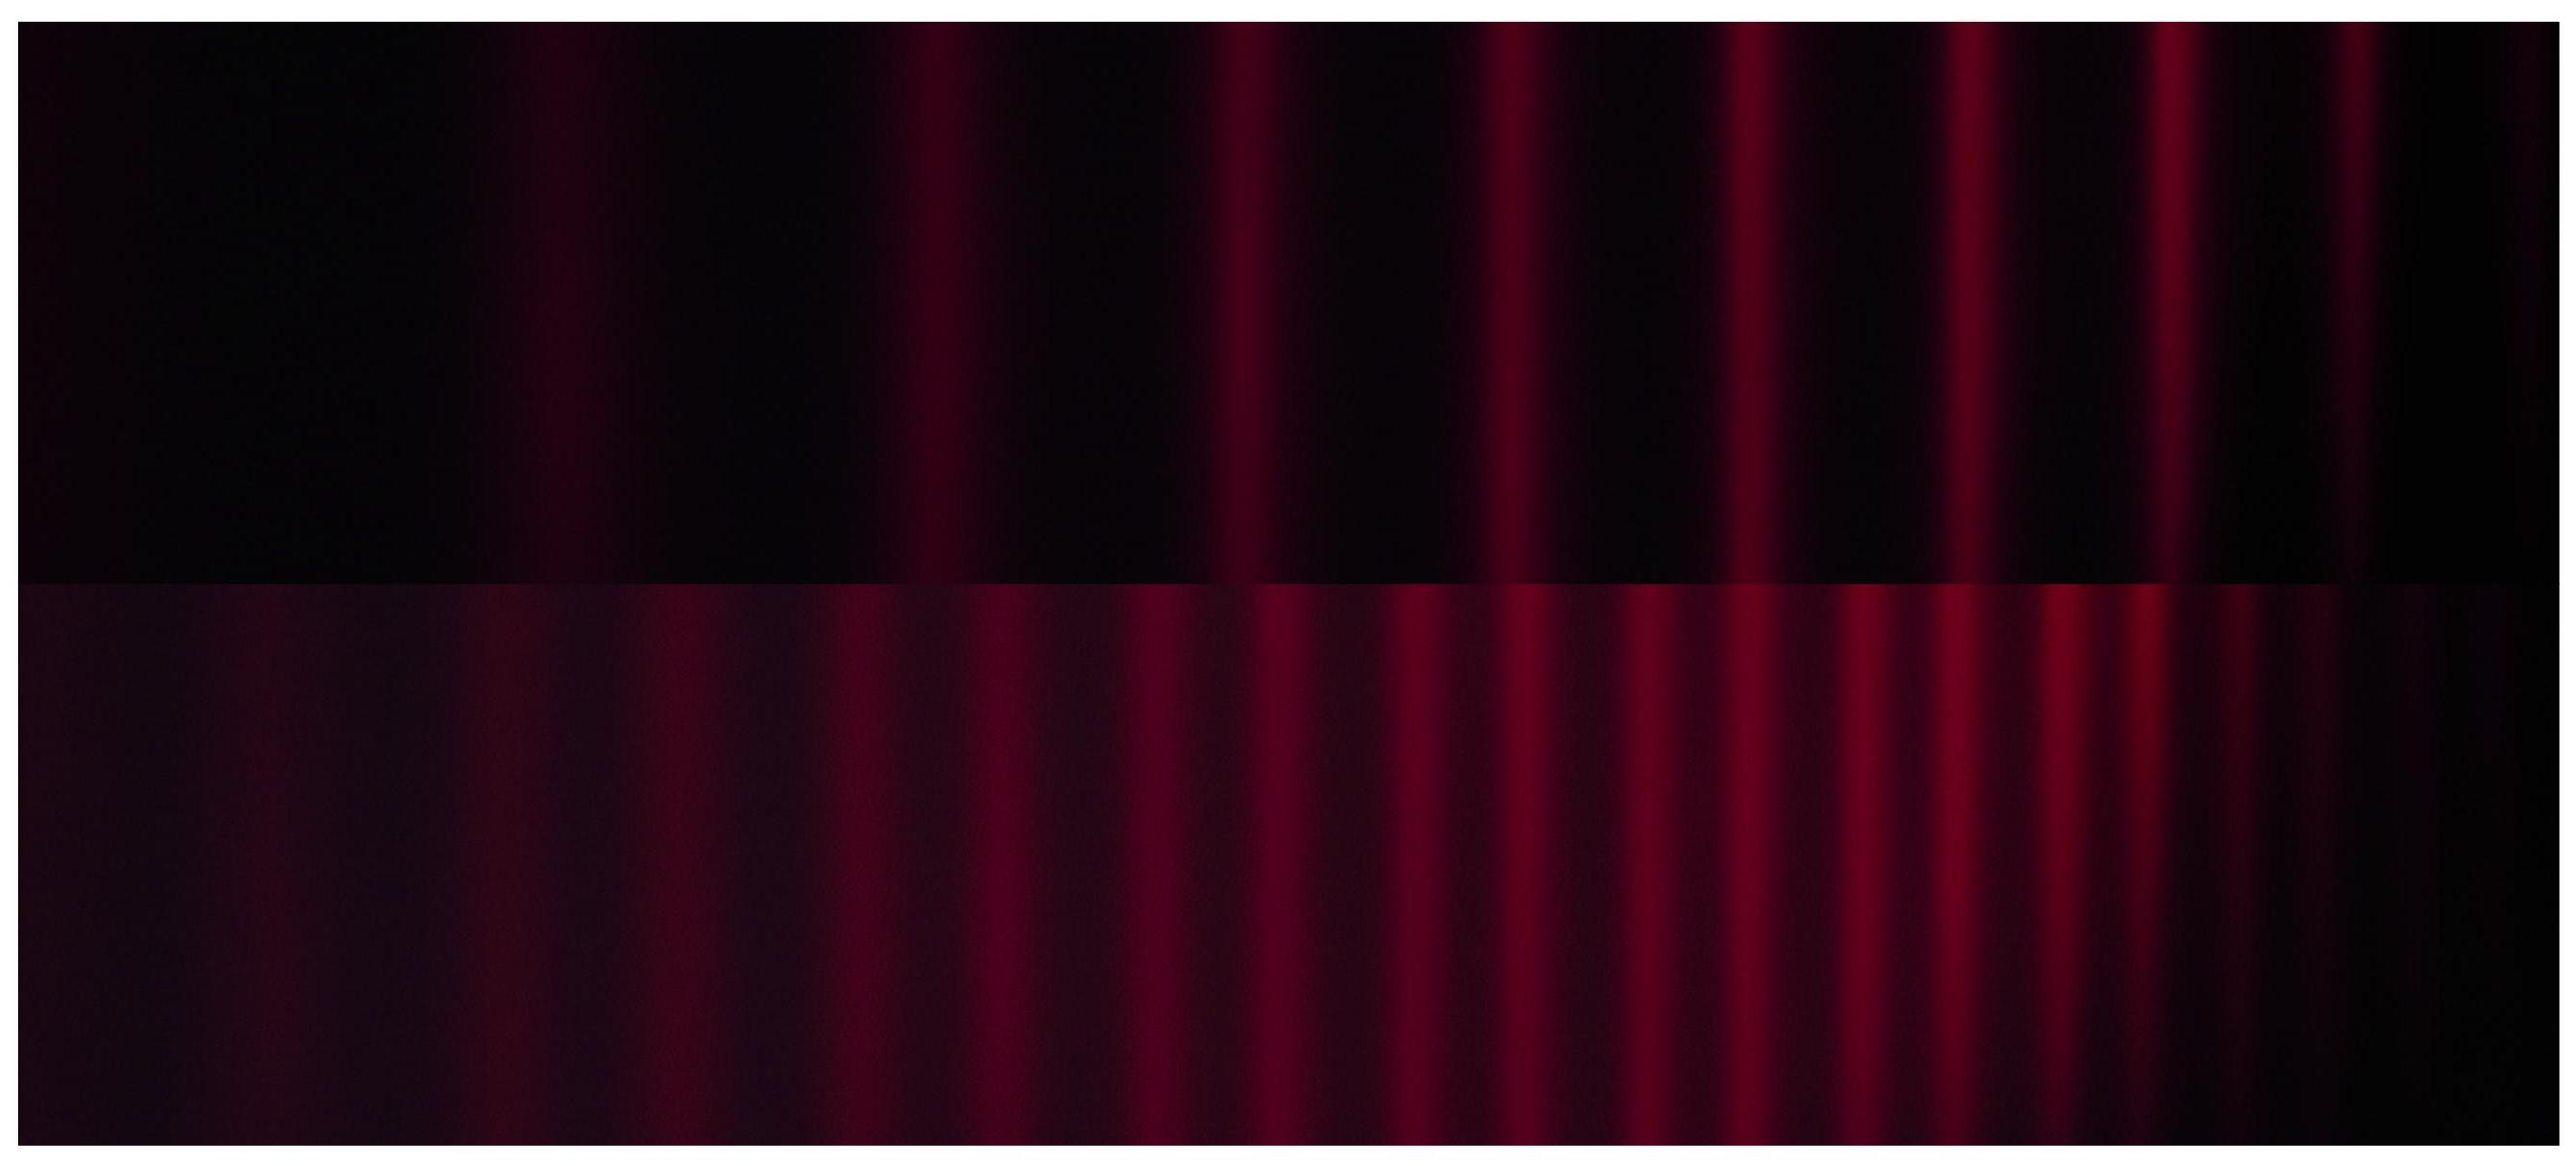
\includegraphics[width=16cm,height=6cm]{Fotos/V27_1.jpg}
	\caption{Interferenzmuster bei Rot (oben B=0, unten B=605 mT)}
	\label{plot:1}
\end{figure}
    
 Dabei entspricht das obere Muster dem Interferenzmuster bei ausgeschaltetem Magnetfeld (B=0) und das untere Muster den Interferenzmuster bei eingeschaltetem Magnetfeld (B=605 mT). Aus diesen Interferenzmustern wurden mittels Vorschau die in Tabelle \ref{tab:mit3} aufgelisteten Werte ermittelt. Die Wellenlängenverschiebung wurde dabei mittels folgender Formel berechnet:
    
    \begin{equation}
  \label{gl:gleichung}
  \delta\lambda=\frac{\delta s}{2\Delta s} \cdot \Delta\lambda_D
\end{equation}

  \begin{table}[H] 
	\centering
	\caption{Messwerte zur Bestimmung der Wellenlängenänderung} 
	\begin{tabular}{c|c|c|c}

  & $\Delta$ s in px & $\delta s$ in px & $\delta \lambda$ in $10^{-12} m$\\
  \hline 
1 &479&214&10,92 \pm 0,17 \\
2 &339&148&10,68 \pm 0,24 \\
3 &276&131&11,61 \pm0,29 \\
4 &238&104&10,69 \pm0,34 \\
5 &215&95&10,81 \pm 0,37 \\
6 &198&75&9,26 \pm 0,40 \\
7 &174&64&8,99 \pm 0,45 \\
8 &157&60&9,35 \pm 0,50 \\

		
	\end{tabular} 
	  \label{tab:mit3}
\end{table} 

Werden die berechneten Werte gemittelt, ergibt sich für die Wellenlängenverschiebung:

\begin{center}
$\delta \lambda$ = (10,29 \pm 0,21) pm
\end{center}

  \subsection{\texorpdfstring{Bestimmung des Lande-Faktors $g_{12}$ der $\pi$-"Uberg"ange f"ur die blaue Linie}{Bestimmung des Lande-Faktors g_12 der pi-"Uberg"ange f"ur die blaue Linie}}
  
Bestimmung des Lande-Faktors $g_{12}$ der $pi$-Übergänge für die blaue Linie wird nach dem selben Schema wie im Aufgabenteil 4.4. 
  
        \begin{table}[H] 
	\centering
	\caption{Messwerte zur Bestimmung der Wellenlängenänderung} 
	\begin{tabular}{c|c|c|c}

  & $\Delta$ s in px & $\delta s$ in px & $\delta \lambda$ in $10^{-12} m$\\
  \hline 
1&188&92&6,59 \pm 0,24 \\
2&176&84&6,43 \pm 0,25 \\
3&160&72&6,06 \pm 0,28 \\
4&147&63&5,77 \pm 0,30 \\
5&131&58&5,97 \pm 0,34 \\
6&122&52&5,74 \pm 0,36 \\

		
	\end{tabular} 
	  \label{tab:mit4}
\end{table} 

\begin{figure}[h]
	\centering
	
\includegraphics[width=16cm,height=6cm]{Fotos/V27_2.jpg}
	\caption{Interferenzmuster bei Blau (oben B=0, unten B=360 mT)}
	\label{plot:1}
\end{figure}

\begin{center}
$\delta \lambda$ = (6,09 \pm 0,22) pm
\end{center}

\newpage

  \subsection{\texorpdfstring{Bestimmung des Lande-Faktors $g_{12}$ der $\sigma$-"Uberg"ange f"ur die blaue Linie}{Bestimmung des Lande-Faktors g_{12} der sigma-"Uberg"ange f"ur die blaue Linie}}
  
  Bestimmung des Lande-Faktors $g_{12}$ der $sigma$-Übergänge für die blaue Linie wird nach dem selben Schema wie im Aufgabenteil 4.4. 
  
          \begin{table}[H] 
	\centering
	\caption{Messwerte zur Bestimmung der Wellenlängenänderung} 
	\begin{tabular}{c|c|c|c}

  & $\Delta$ s in px & $\delta s$ in px & $\delta \lambda$ in $10^{-12} m$\\
  \hline 
1&178&90&6,81 \pm 0,25 \\
2&172&86&6,73 \pm 0,26\\
3&160&74&6,23 \pm 0,28\\
4&144&58&5,42 \pm 0,30\\
5&124&53&5,76 \pm 0,35\\
6&118&49&5,59 \pm 0,37\\
7&111&44&5,34 \pm 0,39 \\

		
	\end{tabular} 
	  \label{tab:mit5}
\end{table} 

\begin{figure}[h]
	\centering
	
\includegraphics[width=16cm,height=6cm]{Fotos/V27_3.jpg}
	\caption{Interferenzmuster bei Blau (oben B=0, unten B=1020 mT)}
	\label{plot:1}
\end{figure}

\begin{center}
$\delta \lambda$ = (5,99 \pm 0,21) pm
\end{center}


  \subsection{\texorpdfstring{Berechnung der experimentellen Lande-Faktoren $g_{ij}$ aus den Abst"anden $\Delta s$ und $\delta s$ der erhaltenen Aufnahmen}{Berechnung der experimentellen Lande-Faktoren g_{ij} aus den Abst"anden Delta s und delta s der erhaltenen Aufnahmen}}

  $\Delta s$ ist der Abstand der benachbarten Interferentzmaxima in der Aufnahme ohne Magnetfeld, $\delta s$ ist die Breite der Aufspaltung eines Interferenzmaximas, in der Aufnahme mit angelegtem Magnetfeld mit St"arke $B$.
  Damit ergibt sich f"ur den Wellenl"angenunterschied $\delta \lambda$ zwischen den beiden Energieniveaus des "Ubergangs
  \begin{equation}
    \delta \lambda = \frac{1}{2}\frac{\delta s}{\Delta s} \Delta \lambda \; .
  \end{equation}
  Mit
  \begin{align}
    \begin{split}
    \frac{\partial E}{\partial \lambda} = \frac{\delta E}{\delta \lambda} &= \frac{\delta}{\delta \lambda} \frac{hc}{\lambda} = -\frac{hc}{\lambda^2}\\
    \iff \delta E &= \frac{ch}{\lambda^2} \delta \lambda
   \end{split}
  \end{align}
  folgt f"ur den Lande-faktor $g_{12}$ mit der Energieniveaudifferenz $\delta E$/Wellenl"angendifferenz $\delta \lambda$ nach Formel (\ref{g_ij}) der Zusammenhang
  \begin{equation}
    g_{12}=\frac{\delta E}{\mu_BB}=\frac{hc\delta \lambda}{\lambda^2\mu_BB} \; .
  \end{equation}

          \begin{table}[H] 
	\centering
	\caption{Für die Eichung des Magneten aufgenommene Messwerte des Magnetfeldes neben der zugehörigen Stromstärke} 
	\begin{tabular}{c|c|c|c|c}

  $\lambda$ pm & B mT & Übergang & $g_{ij,exp}$& $g_{ij,theo}$\\
  \hline 
643,8 & 632 &$\sigma$&0,84&1\\
480 &360&$\sigma$&1,55&1,25\\
480 &1020 &$\pi$&0,55&0,5\\


		
	\end{tabular} 
	  \label{tab:mit6}
\end{table} 




















\section{Diskussion}
\label{sec:Diskussion}
Für die rote Wellenlänge wird ein Wert von 0,84 gemessen. Das zeigt eine Abweichung von 10\% zum theoretischen Wert. Für die blaue Wellenlänge mit $\pi$-Übergang wird ein Wert von 0,55 gemessen. Das ist eine Abweichung von 10\%. Für die blaue Wellenlänge mit $\sigma$-Übergang wird ein Wert von 1,55 gemessen. Dieser liegt mit einer Abweichung von 24\% sehr weit vom theoretisch errechneten Wert entfernt. Es ist zu vermuten, dass der Fokus der Kamera nicht richtig eingestellt gewesen ist oder auf die Ungenauigkeiten bei der Methode des Auslesens der Werte zurückzuführen.

\section{Literatur}
\label{Literatur}

$[1]$ Skript zu Versuch V27, Physikalisches Fortgeschrittenen Praktikum TU Dortmund

\printbibliography

\end{document}
\fi



\begin{document}

\begin{frame}
  \titlepage
\end{frame}

\begin{frame}
  \frametitle{Inhaltsverzeichnis}
  \tableofcontents
\end{frame}

\section{Einleitung}
  \begin{frame}
    \frametitle{Deine mudda}
    Deine mudda ist adipositas:
    \begin{equation}
      \sin(x)=\int_0^{\infty} \exp(\text i \pi) \: \text dx
    \end{equation}
  \end{frame}


\end{document}
